\chapter{核心功能模块的实现}

在前面的设计基础上，本章重点讨论科研经费管理系统的具体工程化落地过程。本章将从开发环境的搭建开始，逐步深入到多维分析算法的编码细节、风险预警引擎的实现逻辑，以及如何利用 ECharts 在前端实现数据看板的动态集成。

\section{开发环境与工具的选择}
在实际开发中，本研究构建了一套基于主流 Java 技术栈的工程环境。后端主要依赖 JDK 1.8，项目管理则选用了 Maven 3.6 来处理复杂的依赖关系和自动化构建。核心框架选择了 Spring Boot 2.6.13，这主要是看中了其极佳的稳定性和对各类组件的兼容性；持久层则通过 MyBatis-Plus 3.5.3.1 对数据库底层的存取进行了封装。

前端部分采用的是 Node.js 20.x 环境，并利用构建工具 Vite 显著缩短了开发时的热更新时间。界面逻辑基于 Vue 3.5 的组合式 API 开发，并配合 Element Plus 保证了交互组件的规范感。数据库则选用了性能稳健的 MySQL 8.0。这些工具的整合，为后续复杂功能的实现提供了可靠的基础。

\section{核心业务与分析逻辑的落地}

\subsection{项目生命周期的状态驱动实现}
为了让项目的进度变得直观，本系统设计了一套由 6 级内部状态驱动的生命周期管理机制。在数据库中，项目状态从草案（0）到已结项（4）不等。前端在接收到后端返回的状态枚举后，会利用 Vue 的计算属性动态匹配对应的彩色标签。比如“执行中”显示为绿色，“待审批”显示为黄色，这样科研人员一眼就能看清自己负责的所有项目正处于什么阶段。

\begin{figure}[htbp]
    \centering
    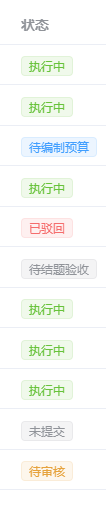
\includegraphics[width=0.7\textwidth,totalheight=0.3\textheight,keepaspectratio]{figures/project_tags.png}
    \caption{基于状态机的项目生命周期可视化标签}
    \label{fig:project_tags}
\end{figure}

\subsection{角色差异化的智能标签生成算法}
系统在列表服务层实现了一套角色感知的智能标签（Intelligent Tags）生成算法。虽然底层计算逻辑统一，但在业务表现与用户交互逻辑上，针对“科研人员”与“管理人员”进行了差异化的业务语义定义。

\subsubsection{科研人员维度：引导型与预警型标签}
对于科研人员，标签的核心功能是“进度引导”与“多级风险感知”。预警标签根据执行偏差 $\Delta$（$\Delta = \text{TimeRate} - \text{FundRate}$）的程度划分为不同等级：
\begin{enumerate}
    \item \textbf{严重风险标签（红色）}：包括“严重滞后”（$\Delta > 50\%$）与“支出异常”（$\Delta < -50\%$）。前者提示项目可能停滞，后者提示存在短时间超额开支风险。
    \item \textbf{常规预警标签（橙色）}：包括“进度滞后”（$\Delta > 30\%$）与“支出偏快”（$\Delta < -30\%$）。
\item \textbf{资源风险标签（软预警）}：如“余额告急”（剩余预算不足 10\%），该标签仅作为**事前提示**，指引科研人员在报销前进行自我核查，避免无效申报。
\end{enumerate}

\subsection{经费报销的分布式余额硬拦截机制}
真正的财务安全由后端 \texttt{FundExpenditureServiceImpl} 的“硬拦截”机制保障。在报销申请提交时刻，系统会通过严格的额度校验算法，对不合规行为进行物理阻断。

\begin{lstlisting}[language=Java, caption={后端预算超支硬拦截逻辑}]
// 1. 获取该科目已通过的支出总额 (status = 1)
BigDecimal usedAmount = approvedExpenditures.stream()
    .map(FundExpenditure::getAmount)
    .reduce(BigDecimal.ZERO, BigDecimal::add);

// 2. 校验拦截：若当前申请金额超过可用余额，触发异常抛出
if (expenditure.getAmount().compareTo(budgetLimit.subtract(usedAmount)) > 0) {
    throw new RuntimeException("报销失败：该科目余额不足。决策建议：请申请预算调剂或核对报销流水。");
}
\end{lstlisting}

\subsubsection{管理人员维度：监控型与任务型标签}
对于管理人员，标签系统演变为“审批任务驱动器”与“资产审计传感器”。管理员可直接识别需要介入的业务节点：
\begin{enumerate}
    \item \textbf{任务驱动标签}：如“待审核”，直接对应待处理的立项或结题审批任务；“待启动”，对应已通过初审但尚未完成预算编制的项目。
    \item \textbf{资产风险标签}：如“逾期”，标识必须进行财务清算的异常项目，支撑管理员进行强制结账操作。
    \item \textbf{合规监控标签}：如“执行滞后”与“余额告急”，用于宏观调控全校经费执行进度，防范学术呆账。
\end{enumerate}

\begin{lstlisting}[language=Java, caption={后端 Service 层全量标签生成逻辑}]
// 根据 status 枚举值生成流程驱动标签
if (status == 1) tags.add("待审核"); // 驱动管理员审批流
if (status == 2) tags.add("待启动"); // 监控立项后预算编制进度

// 基于日期扫描生成资产审计标签
if (now.isAfter(project.getEndDate())) {
    tags.add("逾期"); // 提示进行强制财务清算
}
\end{lstlisting}

\begin{figure}[htbp]
    \centering
    
\includegraphics[width=0.7\textwidth,totalheight=0.3\textheight,keepaspectratio]{figures/intelligent_tags_researcher.png}
    \caption{科研人员视角下的智能风险标签展示}
    \label{fig:intelligent_tags_researcher}
\end{figure}

\begin{figure}[htbp]
    \centering
    
\includegraphics[width=0.7\textwidth,totalheight=0.3\textheight,keepaspectratio]{figures/intelligent_tags_admin.png}
    \caption{管理人员视角下的智能标签表现（侧重审批任务与全局监控）}
    \label{fig:intelligent_tags_admin}
\end{figure}

\subsection{多维度经费统计聚合逻辑}
系统决策支持的核心在于对海量报销流水的实时聚合。在 \texttt{FundStatisticsServiceImpl} 中，系统通过 Lambda 表达式对不同维度的经费进行切片统计。

\begin{lstlisting}[language=Java, caption={核心执行率计算算法}]
private BigDecimal calculateRate(BigDecimal spent, BigDecimal budget) {
    if (budget.compareTo(BigDecimal.ZERO) > 0) {
        // 使用 HALF_UP 舍入模式确保财务计算精度
        return spent.divide(budget, 4, RoundingMode.HALF_UP)
                    .multiply(new BigDecimal("100"));
    }
    return BigDecimal.ZERO;
}
\end{lstlisting}

\subsection{经费支出的“余额硬拦截”与预警}
在支出记录模块，系统通过 AOP 拦截与实时余额检索，实现了经费报销的动态平衡控制。当报销金额超过分项余额、或项目已逾期时，前端会实时反馈高亮警告。

%此处需要一张“报销录入页-余额预警”的截图
%建议操作：在报销录入界面，选择一个余额不足的项目录入大额支出，截取页面顶部的红色/黄色警告框，命名为 expenditure_alert.png
\begin{figure}[htbp]
    \centering
    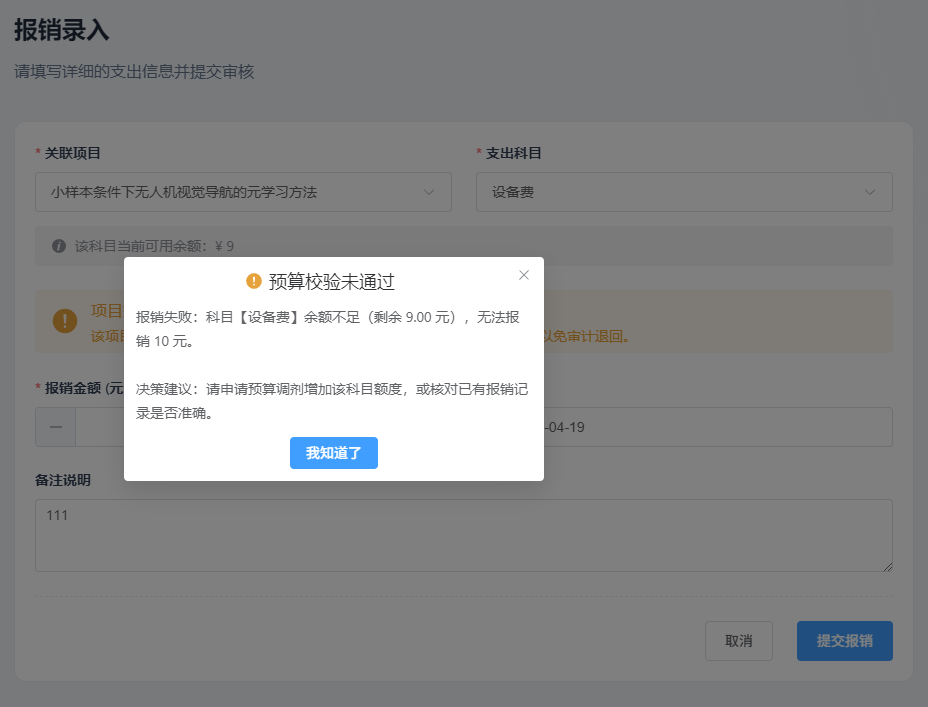
\includegraphics[width=0.7\textwidth,totalheight=0.3\textheight,keepaspectratio]{figures/expenditure_alert.png}
    \caption{基于预算阈值的报销录入硬拦截机制}
    \label{fig:expenditure_alert}
\end{figure}

\subsection{智能助手风险扫描机制}
“智能助手”模块是本系统的技术亮点之一，它通过主动巡检模式识别潜在的财务风险。其实现逻辑如下代码所示：

\begin{lstlisting}[language=Java, caption={智能助手预警巡检逻辑}]
// 扫描执行进度滞后 (时间进度 - 经费执行率 > 10\%)
for (ExecutionRateVO rateVO : rates) {
    ResearchProject rp = projectMapper.selectById(rateVO.getProjectId());
    if (rp != null && rp.getStatus() == 4) { // 仅针对执行中项目
        BigDecimal timeProgress = rateVO.getTimeProgress();
        BigDecimal execRate = rateVO.getRate();
        // 核心判别式：当时间进度领先经费执行率 10\% 以上时触发
        if (timeProgress.subtract(execRate).compareTo(new BigDecimal("10")) > 0) {
            advices.add(AssistantAdviceVO.builder()
                .title("执行进度提醒")
                .content("项目经费执行显著滞后于时间进度，建议加快实施。")
                .type("warning").build());
        }
    }
}
\end{lstlisting}

%此处需要一张“智能助手侧边栏”的运行截图
%建议操作：登录科研人员账号，点击右下角紫色AI小球展开抽屉，截图命名为 assistant.png
\begin{figure}[htbp]
    \centering
    
\includegraphics[width=0.6\textwidth,totalheight=0.3\textheight,keepaspectratio]{figures/assistant.png}
    \caption{智能助手风险建议面板}
    \label{fig:assistant}
\end{figure}

\subsection{全校执行风险监控看板}
针对管理层，系统实现了“全校风险监控”功能。该看板集成了多维维度的全量数据扫描能力，管理员可通过“视角切换器（Researcher Selector）”下钻查看特定科研人员的项目细节，实现了从“宏观总览”到“微观审计”的无缝衔接。

%此处需要一张合并截图：包含顶部的风险卡片，且同时展开右上角的“监控视角”下拉列表
%截图命名为 admin_monitor_combined.png
\begin{figure}[htbp]
    \centering
    
\includegraphics[width=0.8\textwidth,totalheight=0.35\textheight,keepaspectratio]{figures/admin_monitor_combined.png}
    \caption{管理端监控视角切换与全校风险仪表盘集成界面}
    \label{fig:admin_monitor_combined}
\end{figure}

\subsection{经费执行与自然时间进度的对比分析}
决策支持系统的核心技术亮点在于“经费执行率”与“项目时间进度”的二元对比分析。系统摒弃了孤立的数据展示，通过将两组数据投射到同一坐标系，直观揭示执行异常。

\begin{lstlisting}[language=Java, caption={自然时间进度计算算法}]
// 计算时间进度 (已过天数 / 总天数)
if (project.getStartDate() != null && project.getEndDate() != null) {
    long totalDays = ChronoUnit.DAYS.between(project.getStartDate(), project.getEndDate());
    if (totalDays > 0) {
        long elapsedDays = ChronoUnit.DAYS.between(project.getStartDate(), LocalDate.now());
        // 钳制在 0-100% 之间，防止未开始或已结题导致的数据畸变
        long effectiveElapsed = Math.max(0, Math.min(totalDays, elapsedDays));
        BigDecimal progress = new BigDecimal(effectiveElapsed)
                .divide(new BigDecimal(totalDays), 4, RoundingMode.HALF_UP)
                .multiply(new BigDecimal("100"));
        rateVO.setTimeProgress(progress);
    }
}
\end{lstlisting}

该算法保证了进度的客观性。当前端检测到执行率 $\text{FundRate}$ 显著低于 $\text{TimeProgress}$ 时，系统会自动触发“执行滞后”预警，为管理人员提供深度的干预参考。

%此处需要一张“经费执行与进度对比”的重叠条形图截图
%建议操作：截图看板中那个带有淡灰色背景柱（时间）和彩色前景柱（经费）的对比图，命名为 execution_compare.png
\begin{figure}[htbp]
    \centering
    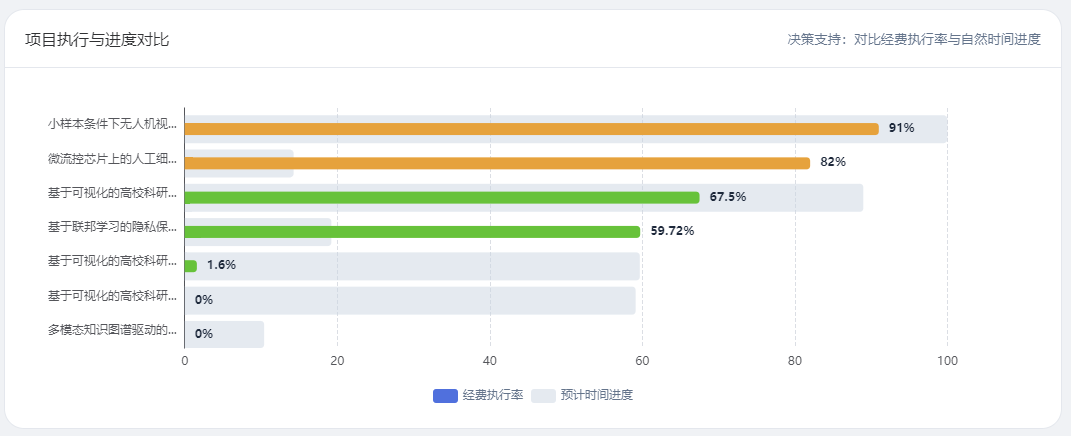
\includegraphics[width=0.75\textwidth,totalheight=0.35\textheight,keepaspectratio]{figures/execution_compare.png}
    \caption{经费执行率与自然时间进度的双维度对比分析图}
    \label{fig:execution_compare}
\end{figure}

\subsection{月度支出趋势与未来预测算法}
系统不仅展示历史数据，还利用简单的线性平滑模型对次月支出进行预测。预测逻辑取最近三个月的有效支出均值。

\begin{lstlisting}[language=Java, caption={趋势预测核心逻辑}]
// 基于近三个月均值进行滚动预测
List<BigDecimal> last3Months = recentValidAmounts.stream()
    .limit(3).collect(Collectors.toList());
if (!last3Months.isEmpty()) {
    forecastAmount = last3Months.stream()
        .reduce(BigDecimal.ZERO, BigDecimal::add)
        .divide(new BigDecimal(last3Months.size()), 2, RoundingMode.HALF_UP);
}
\end{lstlisting}

\section{可视化仪表盘的前端集成}

\subsection{ECharts 动态数据绑定设计}
在前端 \texttt{DashboardView.vue} 中，系统通过响应式配置项（Options）实现了数据看板的实时渲染。特别是“经费执行率与时间进度”的对比图，采用了重叠条形图设计。

\begin{lstlisting}[language=Java, caption={ECharts 双维度对比图绑定配置}]
// 利用负间隔 barGap 实现经费填充背景进度条的效果
series: [
  {
    name: '预计时间进度',
    type: 'bar',
    data: progresses, // 后端推送的 timeProgress 数组
    itemStyle: { color: 'rgba(203, 213, 225, 0.5)' }
  },
  {
    name: '经费执行率',
    type: 'bar',
    barGap: '-72%', // 关键：实现中心重叠对比
    data: rates,
    itemStyle: { 
        color: (p) => p.value >= 100 ? '#F56C6C' : '#67C23A' 
    }
  }
]
\end{lstlisting}

%此处需要一张“月度支出趋势与预测”的图表截图
%建议操作：查看看板底部的折线图，包含虚线预测部分，截图命名为 trend_forecast.png
\begin{figure}[htbp]
    \centering
    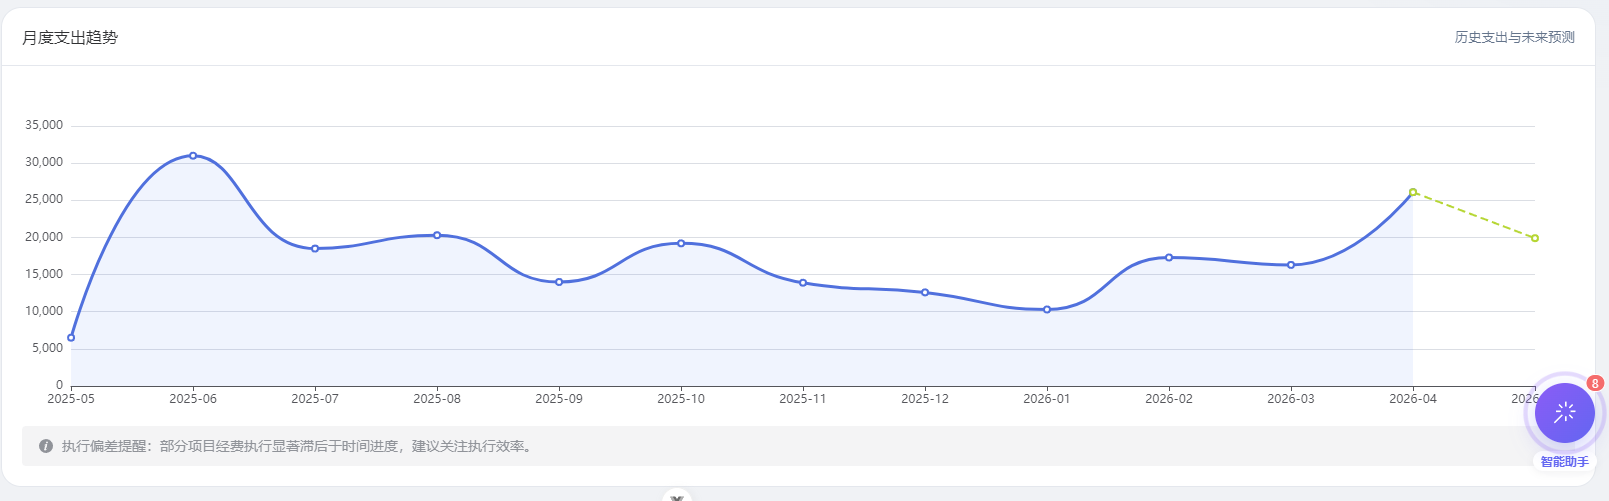
\includegraphics[width=0.7\textwidth,totalheight=0.3\textheight,keepaspectratio]{figures/trend_forecast.png}
    \caption{月度支出趋势与未来月份预测可视化}
    \label{fig:trend_forecast}
\end{figure}

%此处需要一张“经费分类占比-饼图”的截图
%建议操作：截取看板中的“分类支出占比”饼图，命名为 category_share_pie.png
\begin{figure}[htbp]
    \centering
    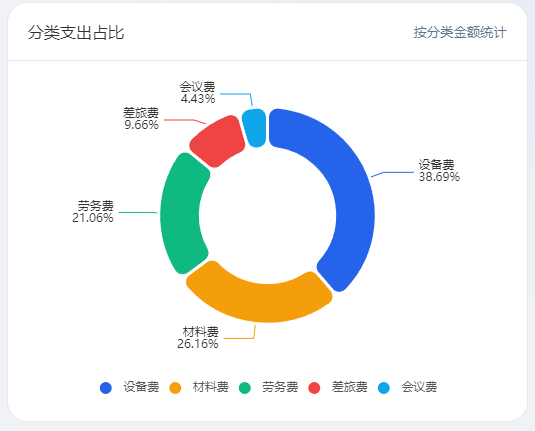
\includegraphics[width=0.6\textwidth,totalheight=0.3\textheight,keepaspectratio]{figures/category_share_pie.png}
    \caption{多维度经费支出占比决策分析}
    \label{fig:category_share_pie}
\end{figure}

\section{本章小结}
本章详细讨论了科研经费管理系统的核心代码实现与可视化集成工作。通过后端基于 Spring Boot 的服务编排和前端基于 ECharts 的数据驱动，本研究成功构建了从底层数据采集、多维风险扫描到顶层决策展示的完整工程路径。特别是在“拦截机制”与“智能助手预警模型”上的具体落地，证明了该系统在高校财务数字化转型实践中的可行性。
